% This is the Oregon State University LaTeX template. To the best of my
% knowledge, most of the work was done by those acknowledged in beavtex.cls.

%%
%% Preamble
%%
% \documentclass{<something>} must begin each LaTeX document
\documentclass[double,12pt]{beavtex}
% Added by CII
\usepackage{graphicx,latexsym, array, wrapfig}
\usepackage{amsmath}
\usepackage{amssymb,amsthm}
\usepackage{longtable,booktabs,setspace}
\usepackage[hyphens]{url}
\usepackage[colorlinks = true, 
			urlcolor = blue,
			linkcolor = black,
			citecolor = black,
			anchorcolor = black]{hyperref}
\usepackage{lmodern}
\usepackage{float}
\floatplacement{figure}{H}
% End of CII addition
\usepackage{rotating} % Package added to allow the rotation of figures and chart
                      % on a page, {sidewaysfigure} command
\usepackage{tablefootnote} % Packaged added to allow footnotes in the tabular
                           % environment, use \tablefootnote command

% This has to do with a default pandoc thing
% http://tex.stackexchange.com/a/258486/77699
\providecommand{\tightlist}{%
  \setlength{\itemsep}{0pt}\setlength{\parskip}{0pt}}

% Added by CII (Thanks, Hadley!)
% Use ref for internal links
\renewcommand{\hyperref}[2][???]{\autoref{#1}}

\def\sectionautorefname{Section}
\def\subsectionautorefname{Subsection}
% End of CII addition

% Added by CII
\usepackage{caption}
\captionsetup{width=5in}
% End of CII addition

\title{Response of Stream Macroinvertebrate Community to Canopy-opening
Manipulations} % {An Analysis of Something}
\author{Cedar Mackaness} % {Joseph A. Student}
\degree{Honors Baccalaureate of Science} % {Master of Science}
\doctype{Thesis}
\submitdate{January 1, 2013} % {January 1, 2013}
\commencementyear{2020} % {2013}

\department{Environmental Science} % {Nuclear Engineering and Radiation Health Physics}

\depttype{College of Earth, Ocean and Atmospheric Sciences} % {School}

\depthead{Dave Lytle} % {Director}

\major{Environmental Science} % {Radiation Health Physics}

\advisor{Dana Warren} % {Jane R. Professor}

\abstract{Stream light availability is an important factor influencing aquatic
food webs. In forested headwaters, stream algal production is highly
light-limited, and an increase in light often enhances benthic algal
growth, which in turn increases food availability for primary consumers
in the stream. In forested headwater streams, light availability is
almost entirely mediated by the canopy structure of stream-side
vegetation. Over the last century, many streamside forests in the
Pacific Northwest were heavily harvested, leaving dense second-growth
vegetation for the time being. Under current conditions we would expect
dense closed canopies, little primary production, and a low abundance of
invertebrates that feed on stream algae. We investigated the response of
benthic periphyton, stream macroinvertebrates, and prey consumption by
trout to a release from light limitation in a paired-reach study design.
We hypothesized that increases in light availability would have a
positive response on grazing macroinvertebrates due to elevated algal
production, and predicted that this change in community structure would
be reflected in the diets of trout. We found that the presence of a
canopy gap had little influence on the invertebrate community, and this
lack of change was reflected in summer trout diets.}
\acknowledgements{I would like to thank Allison Swartz, Dana Warren and the whole Warren
lab for several years of sometimes-grueling-always-fun work, and the
opportunity and support to work on this thesis project. Additionally, I
would like to acknowledge both Dave Roon and Dave Lytle, my thesis
committee members, for their novel insights and unique perspective. The
parts of this thesis that I am most proud of came about through
collaboration with with all of the people mentioned above, and of course
it was all made possible through the love and encouragement of my
family.}








\begin{document}

\maketitle
\mainmatter


  \chapter*{Introduction}\label{introduction}
  \addcontentsline{toc}{chapter}{Introduction}
  
  In forested systems, streams and their biota are intrinsically linked to
  riparian vegetation (Vannote, Minshall, Cummins, Sedell, \& Cushing
  (\protect\hyperlink{ref-Vannote1980}{1980})). Stream food webs depend on
  direct carbon subsidies from the terrestiral environment in the form of
  both leaf litter and terrestrial invertebrates, but riparian controls on
  stream systems aren't limited to biological inputs. Riparian canopy
  cover also has an indirect effect on stream food webs through the
  control of light available for benthic primary production. In the
  Pacific Northwest (PNW) region of North America, riparian forests have
  changed substantially in the past half century. After a legacy of heavy
  harvesting, riparian forest protections have created dense second-growth
  vegetation along streams in contrast with old-growth forests containing
  multiple canopy gaps. The dense vegetation in these regenerating forests
  decreases light availability and limits benthic primary production. As
  forest stand development continues natural disturbances and individual
  tree mortality will increase canopy heterogeneity through the
  introduction of gaps.To understand how aquatic food webs respond to an
  increase in light associated with canopy gaps, we investigate the
  response of macroinvertebrates and fish feeding to canopy-opening
  manipulations.
  
  Light, and its impact on primary productivity in streams is of
  particular interest because autochthonous carbon can be
  disproportionately represented in consumer biomass relative to its
  availability in many aquatic environments (Lau, Leung, \& Dudgeon
  (\protect\hyperlink{ref-Lau2009}{2009}), McCutchan \& Lewis
  (\protect\hyperlink{ref-McCutchan2002}{2002})). In forested headwater
  systems specifically, basal carbon availability is dominated by leaf
  litter (McCutchan \& Lewis
  (\protect\hyperlink{ref-McCutchan2002}{2002})); however, energetically,
  algae is a higher quality food source and is preferentially assimilated
  into higher trophic levels (Macarelli \& others
  (\protect\hyperlink{ref-Macarelli2011}{2011})). Stream secondary
  production is dominated by aquatic macroinvertebrates which play an
  important role in assimilating and transducing energy to higher trophic
  levels such as insectivorous fish and other vertebrate predators.
  Because macroinvertebrates play a crucial role in mediating food web
  interactions, understanding their community dynamics can provide key
  insights into broader ecosystem functioning. Invertebrates in the
  scraper functional feeding group in particular have evolved specialized
  mouthparts for consuming benthic algal biofilms (periphyton), and
  increases in algal production often elicits a positive response among
  these scraping taxa (@ sources).
  
  Macroinvertebrate community data has historically been used to evaluate
  stream health. Indicies such as the B-IBI or, benthic index of
  biological integrity, rely on total taxa richness and taxa richness of
  key families, such as Plecoptera, Ephemeroptera and Trichoptera, to
  evaluate the biological condition of streams. More broadly, an
  assesement of the whole community can be used to evaluate overall food
  web and ecosystem responses to a multitude of variables. For example,
  studies using nonmetric multidimensional scaling (NMS) have been used to
  assess community responses along a variety of environmental gradients (@
  citations).
  
  The benthic invertebrate community represents the primary food source
  for fish in headwater streams (@ citation). Trout are the dominant fish
  species in many headwater systems across North America, and can
  influence both invertebrate behavior and community structure (@ McIntosh
  and Peckarsky papers -- and maybe something from PNW). In headwater
  streams trout are oportunistic foragers, eating whatever is available in
  their habitat. Cutthroat trout feed from the water column using visual
  cues to capture prey. Because salmonids are visual predators, their
  feeding efficiency can be influenced by light conditions and visibility
  (Wilzbach, Cummins, \& Hall
  (\protect\hyperlink{ref-Wilzbach1986}{1986})), therefore gaps have the
  potential to affect fish feeding not only though potential increases in
  scraper invertebrate food resources, but also by increasing foraging
  efficiency.
  
  Clear cutting and the resultant reach-level increase in stream light can
  increase stream primary and secondary productivity, but increases in
  light also lead to increases in temperature, and cutting to the stream
  edge can increase sediment loads. Given these negative impacts, clear
  cutting along streams is no longer a common practice in the Pacific
  Northwest--even in managed landscapes riparian buffers are left. In
  unmanaged forests, and in these riparian forest buffers, stands are in
  the early to mid-seral stages with dense homogenous canopy cover and low
  stream light (Kaylor, Warren, \& Kiffney
  (\protect\hyperlink{ref-Kaylor2017FS}{2017})). Canopy gaps will begin
  developing naturally along streams as stands mature, and restoration
  efforts focused on emulating natural disturbance may expedite forest
  shifts toward late-succession and old-growth structural conditions
  (Kreutzweiser, Sibley, Richardson, \& Gordon
  (\protect\hyperlink{ref-Kreutzweiser2012}{2012})). While studies on
  reach-scale forest clearing demonstrate a clear response in benthic
  primary producers, invertebrates, and trout to release from light
  limitation, this does not reflect future stream conditions in most
  forested landscapes. As stands progress toward late succesional forest
  structure, localized light patches (rather than large openings) will
  become increasingly prevelant, and have not been widely evaluated.
  
  We hypothesize that canopy gaps will produce a dampened response in
  comparison to clear cutting but, should increase primary production,
  causing the macroinvertebrate community to shift in response to resource
  availability, and resultant changes in the invertebrate community will
  be reflected in the opportunistic foraging of trout.
  
  \chapter*{Methods}\label{methods}
  \addcontentsline{toc}{chapter}{Methods}
  
  \section*{Study location}\label{study-location}
  \addcontentsline{toc}{section}{Study location}
  
  The study consists of five reach pairs on five replicate streams in the
  western Cascade Mountains of Oregon. Each reach pair consisted of one
  treatment reach and one reference reach. Two of the reach pairs (W-100,
  W-113) are located on private Weyerhaeuser Co. land, and three (LOON,
  CHUCK, MCTE) are located on U.S. Forest Service land, one of which
  (MCTE) is situated in the HJ Andrews Experimental Forest. Stream reaches
  were 90 meters in length and treatment gaps were 20 to 40 meters in
  diameter and situated approximately in the middle of treatment reaches.
  Sites had a buffer between stream reach pairs to limit any effects of
  the upstream reach on downstream conditions.
  
  All of the streams are wadeable, fish-bearing streams with bankfull
  widths of 1-8 meters. Fish-bearing streams were purposefully selected to
  provide management-relevant results for key species such as salmonids.
  The streams run through 40-60-year-old riparian forests regenerating
  from previous harvest. These forests have a homogenous canopy structure
  with heavy understory shading, as defined by their early seral stage.
  Small streams were chosen for ease of sampling and to maximize the
  effect of a canopy opening manipulation since small streams may be
  completely shaded by overhead vegetation due to their high edge to area
  ratio.
  
  \begin{table}[t]
  
  \caption{\label{tab:table1}Study site attributes}
  \centering
  \resizebox{\linewidth}{!}{
  \begin{tabular}{lrrrrr}
  \toprule
  Stream & Elevation (m) & Bankful Width (m) & Base flow (L s-1) & Latitude & Longitude\\
  \midrule
  CHUCK & 833.0 & 5.19825 & 21.0 & 43.95362 & -122.1136\\
  LOON & 721.2 & 4.13170 & 12.5 & 43.95362 & -122.1833\\
  MCTE & 867.0 & 2.20000 & 5.0 & 44.25454 & -122.1667\\
  W-100 & 441.0 & 5.39000 & 43.9 & 44.19813 & -122.4930\\
  W-113 & 537.0 & 3.30000 & 9.1 & 44.19289 & -122.5107\\
  \bottomrule
  \end{tabular}}
  \end{table}
  
  \section*{Study Design}\label{study-design}
  \addcontentsline{toc}{section}{Study Design}
  
  The before-after, control-impact (BACI) study design lends itself to
  experimental field studies by accounting for natural variations between
  sites. By taking the ratio of a given variable between the paired
  reaches and comparing the change in the ratio from pre to post-treatment
  years, we account for both spacial and temporal variation. So, going
  forward, a sample unit will refer to a whole stream including both
  treatment and reference reaches because the metric of interest for many
  of our analyses will be the ratio between the two reaches. Therefore we
  have five sample units with two repeated measures, pre and
  post-treatment. To test for effects of the gap treatment, we quantify
  and assess changes in the reach ratio's between the two years. Samples
  were collected during summer 2017 and summer 2018 with pre-treatment
  data gathered during summer 2017 and post-treatment data gathered during
  summer 2018. Canopy gaps were cut in the treatment reach during the
  winter of 2017-18 to permit adequate time for response to the canopy
  manipulation.
  
  \section*{Data Collection}\label{data-collection}
  \addcontentsline{toc}{section}{Data Collection}
  
  \subsection*{Light}\label{light}
  \addcontentsline{toc}{subsection}{Light}
  
  Photosynthetically active radiation (PAR) was estimated from flourescein
  decay rate over a twenty-four hour period following methods in Warren et
  al. Briefly, flourescein dyes were prepared by diluting to 400 g
  L\textsuperscript{-1} with DI water and buffering with 40 g
  L\textsuperscript{-1} of aquarium salt. Once the dye was prepared, we
  filled 3.7mL glass vials and stored them in the dark until deployment.
  At each study reach hree replicate vials were deployed every five
  meters, and retrieved twenty-four hours later. Because flourescence of
  fluorescein changes with temperature (({\textbf{???}})), vials were left
  in the dark until they reached room temperature. Flouresence was then
  measured using a flourometer (Turner Designs, San Jose, California), and
  the twenty-four hour decay rate was converted to photosynthetically
  active radiation (PAR) using the known relationship in
  (({\textbf{???}})).
  
  \subsection*{\texorpdfstring{Chlorophyll
  \emph{a}}{Chlorophyll a}}\label{chlorophyll-a}
  \addcontentsline{toc}{subsection}{Chlorophyll \emph{a}}
  
  In each study reach every ten meters, three ceramic tiles (15 cm x 15cm)
  were placed every 10 meters within a stream reach and left for 6 weeks
  before they were collected to allow periphyton communities to establish.
  Tiles were placed in riffle sections at a depth of 10-25 cm to keep them
  from silting over. All tiles were deployed in mid-July, and the tiles
  were deployed at the control and treatment reaches of each stream at the
  same time to keep within unit measures consistent. After collection,
  tiles were kept in the dark, submerged in water for two hours to avoid
  potential photosasturation issues with the \emph{in situ} chlorophyll
  \emph{a} measurements. Chlorophyll \emph{a} (abbreviated as Chla for the
  remainder of this text) concentrations were then quanitified using a
  BenthoTorch (BBE Moldaenke GmbH), a portable field instrument used for
  the quantification of chlorophyll \emph{a} fluorescence on different
  substrates.
  
  \subsection*{Benthic Invertebrate
  Sampling}\label{benthic-invertebrate-sampling}
  \addcontentsline{toc}{subsection}{Benthic Invertebrate Sampling}
  
  Three benthic invertebrate samples were taken at each stream reach at
  meters 15, 45, 75, or the closest area with non-boulder substrate.
  Samples were collected once per year over the course of one week using a
  Surber sampler with a .09 m\textsuperscript{2} sampling area. Substrate
  was disturbed to a depth of approximately four inches for one minute.
  The sample was then preserved in 95\% ethanol for identification and
  enumeration in the lab.
  
  In the lab, the three benthic samples per reach were combined into a
  single pooled sample for each reach. The pooled sample was then
  subsampled using a Caton tray. Squares \(\frac{1} {30}\) of the area of
  the Caton tray were randomly sampled until the cutoff of 300 individuals
  or greater was reached. Benthic invertebrates were then identified down
  to genus or the lowest taxonomic unit (LTU) for cryptic taxa. Counts
  from subsamples were then converted to densities using the following
  formula:
  
  \begin{equation}
  \frac{1}{3*s*0.09}
  \end{equation}
  
  Where \(s\) is the fraction subsampled, 0.09 is the area of the Surber
  sampler in square meters, and the result is divided by three because
  three samples from meters fifteen, forty-five and seventy-five were
  pooled. Singleton taxa (taxa occurring in only one reach) were removed
  from the original matrix and density values were log transformed to
  reduce the effect of abundant taxa (Chironomidae, \emph{Baetis},
  \emph{Micrasema}) on community relationships by applying the formula
  \(ln(n + 1)\) where \(n\) is the density of a given taxon. The resulting
  matrix of benthic invertebrates at the LTU level of identification (20
  reaches by 64 taxa) was then used for analysis.
  
  Functional feeding groups were assigned using @ Merritt and Cummins
  using only the primary feeding habit of each taxon. For
  
  During Chla tile collection at the two streams with snails as the
  dominant scraper, the number of snails (Juga) and cased caddisfly
  (observed taxa being Uenoidae and Glossosomatidae primarily) on each
  tile were recorded and then removed. before taking readings with a
  BenthoTorch\textsuperscript{TM}.
  
  \subsection*{Trout Diets}\label{trout-diets}
  \addcontentsline{toc}{subsection}{Trout Diets}
  
  Trout diets were collected during the post-treatment year, Trout diets
  were collected during three-pass depletion of fish standing stock and
  were only taken from a subset of fish greater than 100 mm in length.
  Fish were anesthetized using AQUI-S and gastric lavaged. Stomach
  contents were evacuated by inecting water into the fish stomach using a
  piece of small plastic tubing attached to a syringe. Diet samples were
  collected in filter paper and preserved in 95\% ethanol for lab
  processing.
  
  All trout diets were processed (9 to 13 diets per reach) with aquatic
  invertebrates identified down to the family level and terrestrial
  invertebrates identified to order. Because the number of fish dieted in
  each reach varied, the average of all fish diets was used. The resulting
  matrix was then filtered for aquatic species and appended to a matrix of
  2018 benthic invertebrate families (10 reaches by 38 families),
  producing a matrix of 20 sample units (SU's) by 40 families consisting
  of both fish diets and benthic samples. Singleton taxa were then removed
  to create a matrix of combined diet and benthic families of 20 SU's by
  36 families. At this point, the combined matrix was relativized by row
  maxima to compensate for the difference between benthic
  sampling---measured in density per m2---and fish diets.
  
  \section*{Data Analysis}\label{data-analysis}
  \addcontentsline{toc}{section}{Data Analysis}
  
  \subsection*{BACI Analysis}\label{baci-analysis}
  \addcontentsline{toc}{subsection}{BACI Analysis}
  
  The BACI analysis was performed in R (R Core Team
  (\protect\hyperlink{ref-R-base}{2018})), and consisted of calculating
  reach-pair differences by subtracting the control reach value from the
  treatment reach value. Reach ratios were calculated for light, chla,
  total invertebrate density and invertebrate densities by functional
  feeding group. A paired t-test using Welches method was then performed
  for each metric by subtracting the reach ratio from the pre-treatment
  year from the ratio value in the post-treatment year for each stream
  assuming the difference between the two reach ratios should be zero, and
  the degrees of freedom equal four.
  
  \subsection*{Nonparametric Community
  Analysis}\label{nonparametric-community-analysis}
  \addcontentsline{toc}{subsection}{Nonparametric Community Analysis}
  
  Nonparametric analyses were performed in PC-ORD (McCune \& Mefford
  (\protect\hyperlink{ref-PC-ORD}{2016})) and R (R Core Team
  (\protect\hyperlink{ref-R-base}{2018})) using the Vegan package (Oksanen
  et al. (\protect\hyperlink{ref-vegan}{2018})). Blocked multi-response
  permutation procedure (MRBP) was used to assess differences between
  treatment and control reaches in the pre and post treatment years. MRBP
  was followed up with blocked indicator species analysis (ISA) to
  determine underlying taxa driving any grouping detected by MRBP. The
  combined benthic and diet community matrix was subsequently tested for
  any differences between treatment and control reaches and benthic versus
  diet taxa representation using the same MRBP and ISA methods.
  
  To test for any pre-treatment reach differences in 2017, MRBP was run on
  2017 data only with Treatment as the two a priori groups and blocked by
  Stream. The 2018 post-treatment data was then assessed using the same
  MRBP grouping and blocking. MRBP is a nonparametric method used to test
  for differences between groups. This method accommodates paired or
  blocked study designs by accounting for variation related to study
  design variables that have little bearing on the question being
  addressed. In this case, MRBP accounts for any between-stream variation.
  MRBP outputs a p-value for the observed within-group distance (smaller
  distances constituting stronger grouping) by shuffling SU's between
  groups to generate a distribution of possible within-group distances
  (McCune, Grace, \& Urban (\protect\hyperlink{ref-McCune2002}{2002})).
  
  The follow-up ISA calculates an indicator value (IV) for each species.
  The IV is a composite of a taxon's fidelity and exclusivity to a group.
  If a taxon is consistently abundant in one group and never present in
  any other, then it would receive a high IV. Conversely, a taxon rarely
  abundant in SU's of one group and present in other groups would receive
  a low IV (McCune et al. (\protect\hyperlink{ref-McCune2002}{2002})). A
  Monte Carlo test of 1,000 permutations of the taxa matrix was used to
  generate a p-value for each taxon's IV.
  
  Nonmetric multidimensional scaling (({\textbf{???}})) was used to
  visually assess differences between the treatment and control reach
  communities, and quantify the relationship between the synthetic
  community variable and Chla . Sorensen distance was used for both
  ordinations to reduce the impact of outliers. The ordination was rotated
  to maximize the environmental variable BenthoTotal along axis 1. A
  random start was used and the real data were run 250 times to ensure an
  absolute stress minima was reached. A Monte Carlo test with 100
  permutations was used to generate a p-value for the probability of the
  final ordination have a lower than expected p-value by chance.
  
  \subsection*{Analysis of Trout Diets}\label{analysis-of-trout-diets}
  \addcontentsline{toc}{subsection}{Analysis of Trout Diets}
  
  Trout diets were collected in the post-treatment year, which limits
  analysis to a comparison of reference and treatment reaches without the
  BACI control on inherent reach differences. We performed paired t-tests
  for the abundance of each functional feeding group represented in the
  diets of trout in the reference and the treatment reach, and on the
  modified Ivlev's selectivity index (as defined in ({\textbf{???}})) for
  each FFG.
  
  \chapter*{Results}\label{results}
  \addcontentsline{toc}{chapter}{Results}
  
  \section*{Light and Chlorophyll}\label{light-and-chlorophyll}
  \addcontentsline{toc}{section}{Light and Chlorophyll}
  
  In 2017, before treatment, the average daily PAR reaching the stream
  benthos among the five streams was consistently low in both reference
  and treatment reaches and there was an average difference between the
  treatment and reference reach of -0.163 mol m\textsuperscript{-2}
  day\textsuperscript{-1}. In 2018, after gaps were cut, light went up by
  2.604 mol m\textsuperscript{-2} day\textsuperscript{-1} on average in
  the treatment reach compared to the reference reach (Figure 1) resulting
  in a final yearly difference between reach differences of 2.767 mol
  m\textsuperscript{-2} day\textsuperscript{-1} (p-value = 0.01862,
  t-value = -3.8296).
  
  Again, for chlorophyll \emph{a}, values across all sites in the
  pre-treatment year were low (mean = 0.095 ug cm\textsuperscript{-2}),
  and there was little difference between reaches. After gaps were cut in
  the post-treatment year, Chla values went up by 0.44 ug
  cm\textsuperscript{-2} in the gap reach, and only 0.175 ug
  cm\textsuperscript{-2} in the reference reach (final BACI difference =
  0.265 ug cm\textsuperscript{-2}, p-value = 0.0017).
  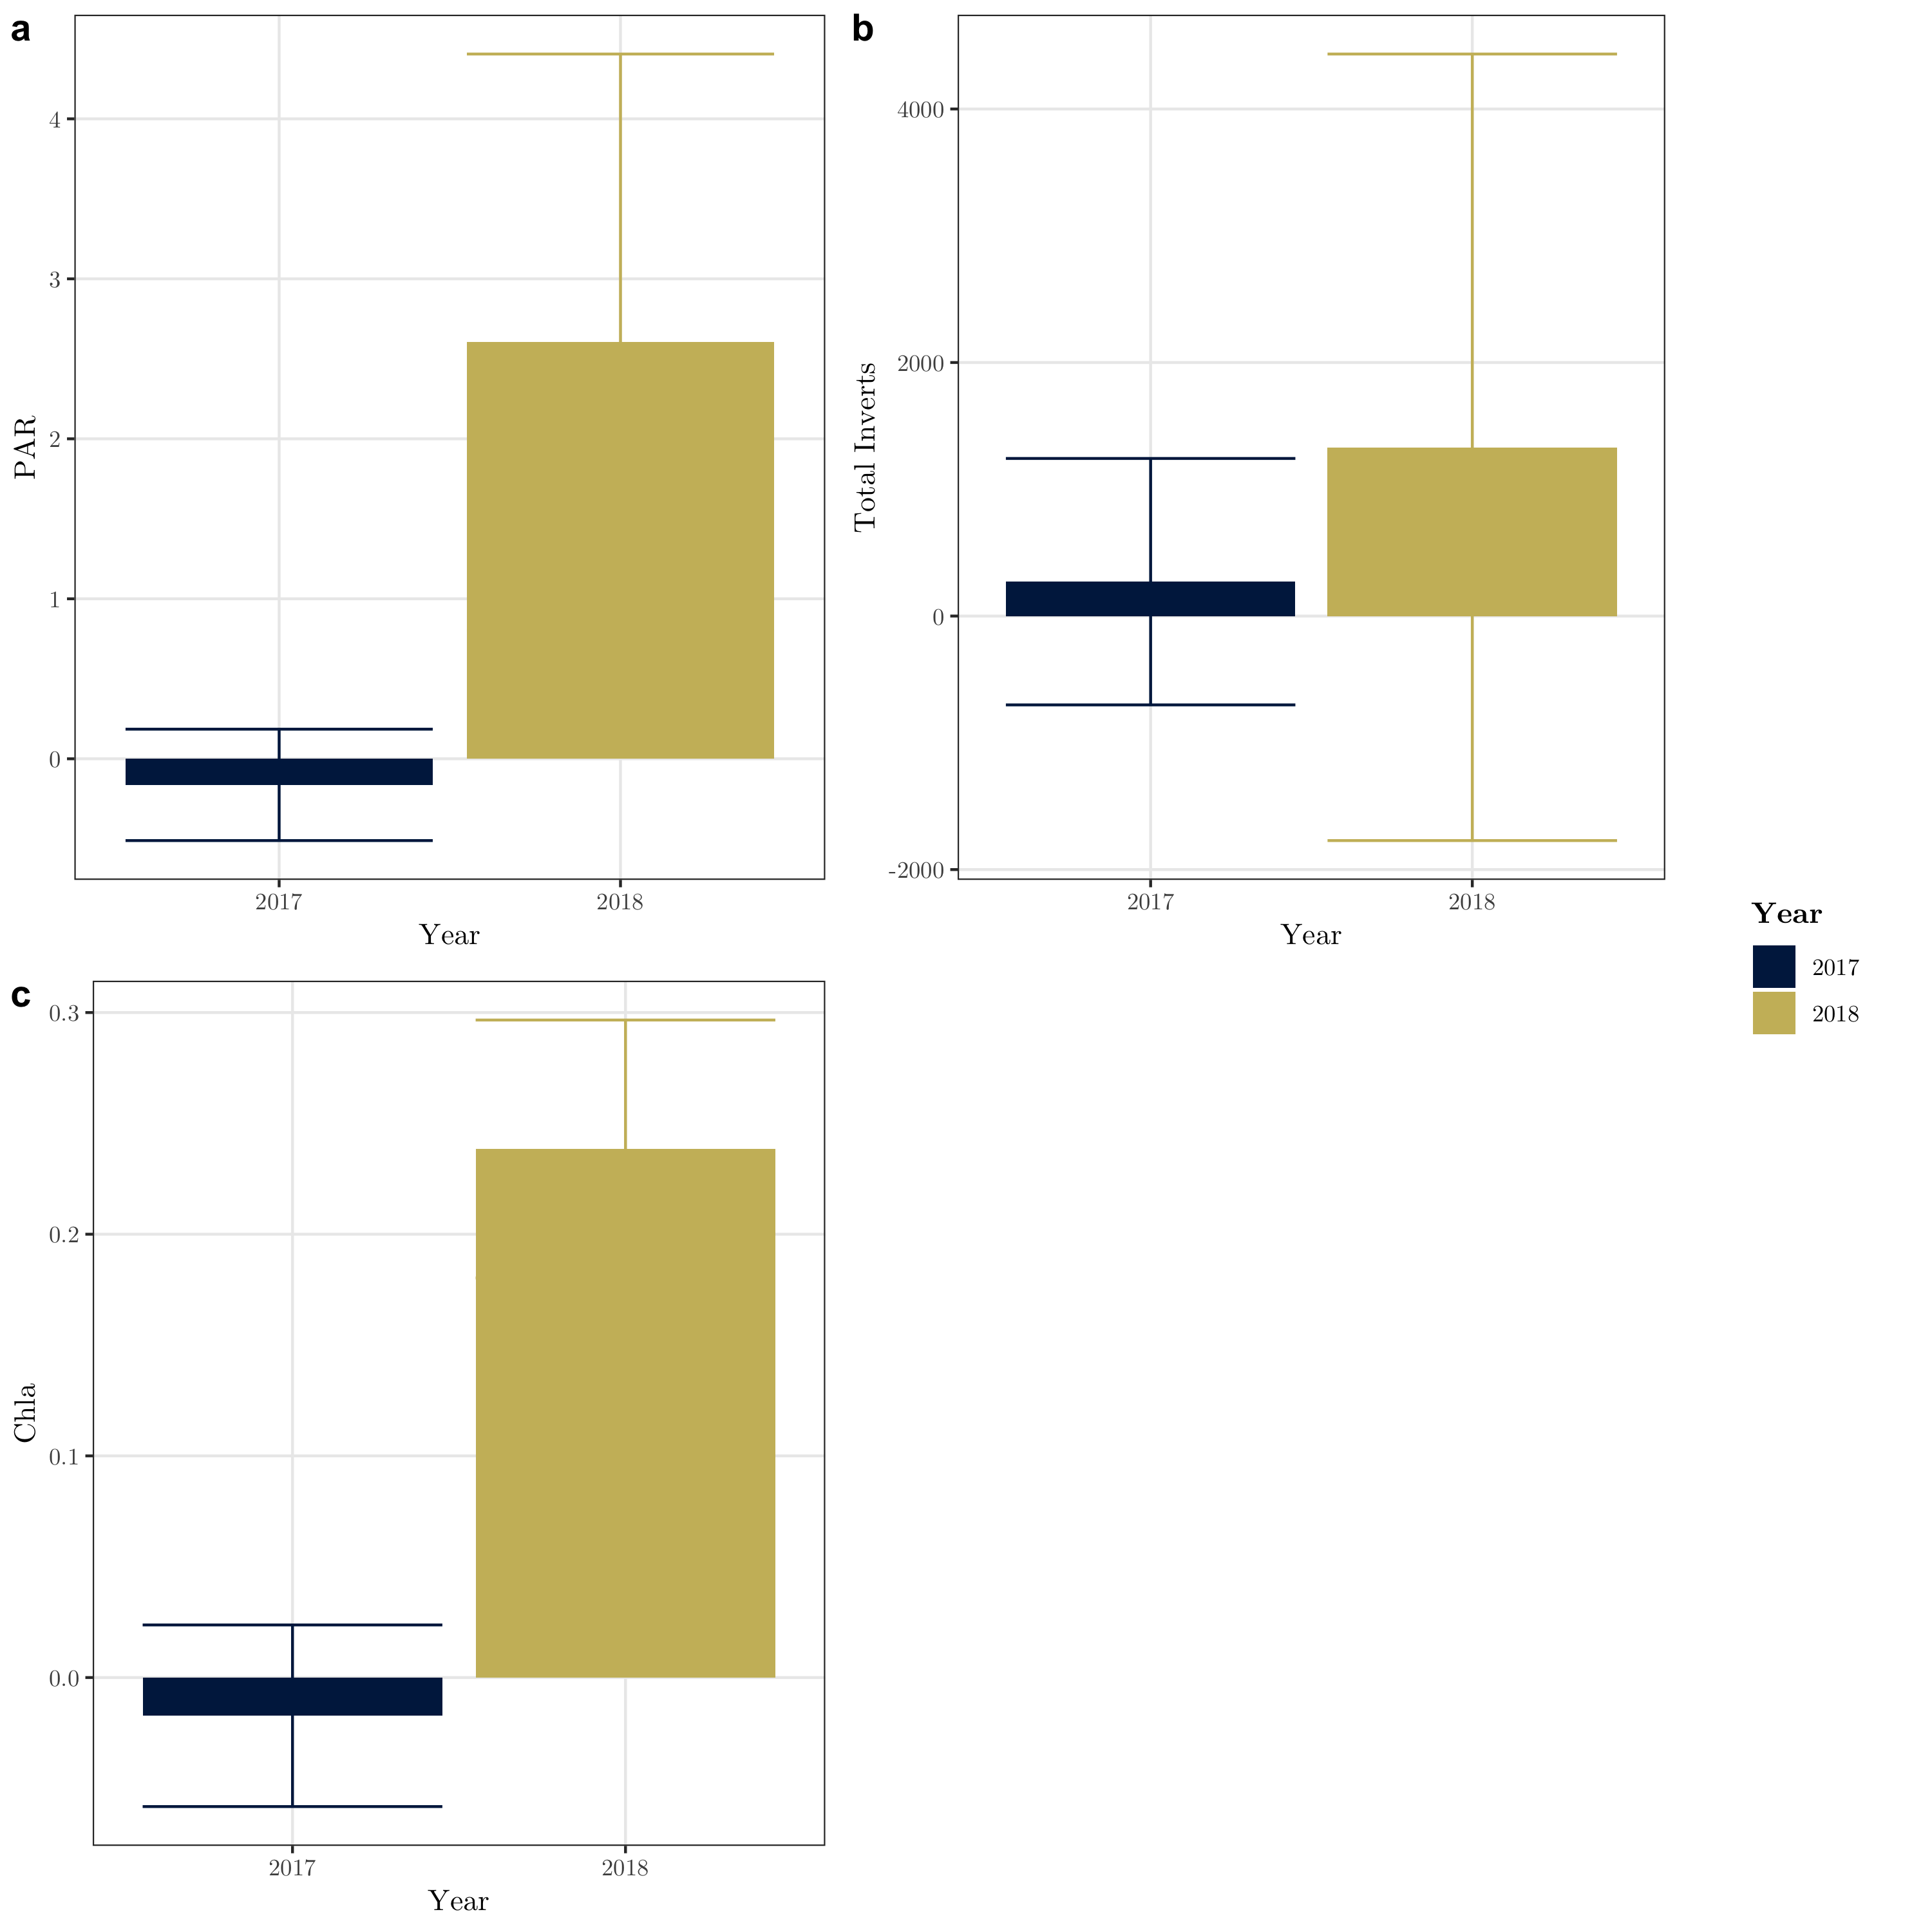
\includegraphics[width=4.16667in]{Figures/Vars_Reach_Diffs.png}
  
  \section*{\texorpdfstring{\emph{Juga} on
  Tiles}{Juga on Tiles}}\label{juga-on-tiles}
  \addcontentsline{toc}{section}{\emph{Juga} on Tiles}
  
  The average density of \emph{Juga} on tiles between the two streams with
  \emph{Juga} present in the pre-treatment year was \textbf{XXX} snails
  per m\^{}2 with little difference between the control and treatment
  reaches. In the post treatment year the average snail density in the
  treatment reach increased by \textbf{XXX} snails per m\^{}2, whereas
  snail density in the control reach only increased by \textbf{XXX}. The
  ratio between
  
  \section*{Benthic Invertebrate
  Community}\label{benthic-invertebrate-community}
  \addcontentsline{toc}{section}{Benthic Invertebrate Community}
  
  There was little difference between benthic invertebrate communities in
  the treatment and reference reaches in the pre-treatment year (MRBP: A =
  0.041, p = 0.071), or the post-treatment year (A = -0.022, p = 0.838).
  The results from the NMS ordinations support the results of the MRBP
  (Figure 2). 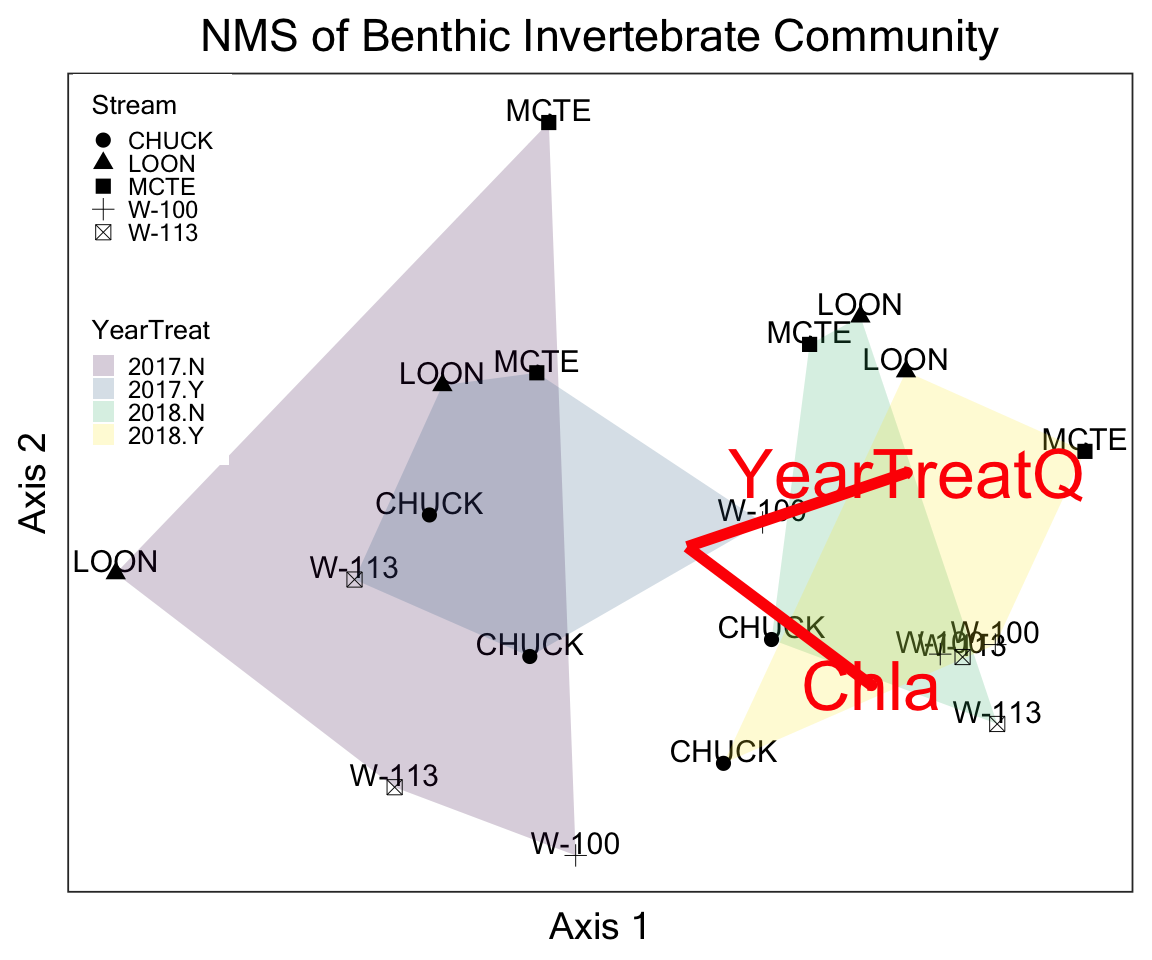
\includegraphics[width=4.16667in]{Figures/NMS Benthic-1.png}
  The NMS ordination of benthic invertebrates converged on a 2D solution
  with a final stress of 12.031. BenthoTotal (total chlorophyll values
  from the Bentho TorchTM) and YearTreatQ (a binary variable coded with
  1's for 2018 treated reaches and 0's for all other reaches) with
  positive r values with axis 1 of 0.272 and 0.298 for YearTreatQ, and
  0.304 and 0.41 for BenthoTotal respectively. The mantel test showed a
  similar level of relatedness between the original family and LTU
  distance matrices (r = 0.986, p = 0.001)
  
  \section*{Invertebrate Functional Feeding
  Groups}\label{invertebrate-functional-feeding-groups}
  \addcontentsline{toc}{section}{Invertebrate Functional Feeding Groups}
  
  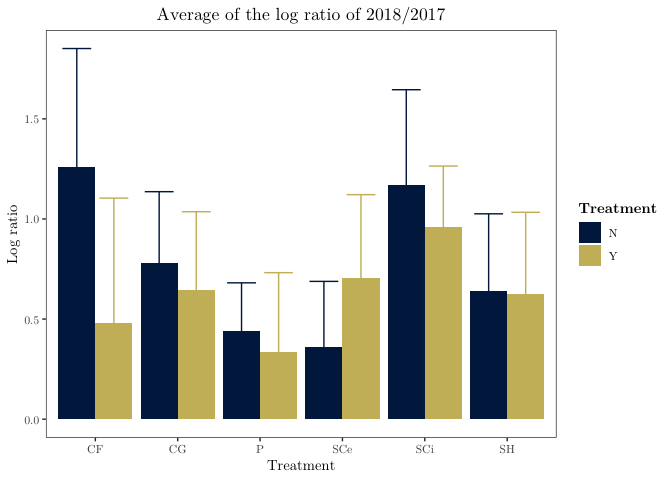
\includegraphics[width=4.16667in]{Figures/AvgFFGratio-1.png}
  
  \begin{table}[t]
  
  \caption{\label{tab:ffgtable}BACI t-test results for various metrics}
  \centering
  \begin{tabular}{lrr}
  \toprule
  FFG & t-value & p-value\\
  \midrule
  SH & 0.0711617 & 0.9450224\\
  P & 0.5161519 & 0.6224931\\
  SCe & -1.5465440 & 0.1624379\\
  CG & 0.5978468 & 0.5666133\\
  SCi & 0.8552979 & 0.4216123\\
  \addlinespace
  CF & 2.1321982 & 0.0656781\\
  All Bugs & 0.8400000 & 0.4300000\\
  \bottomrule
  \end{tabular}
  \end{table}
  
  \section*{Trout Diet}\label{trout-diet}
  \addcontentsline{toc}{section}{Trout Diet}
  
  \begin{figure}[htbp]
  \centering
  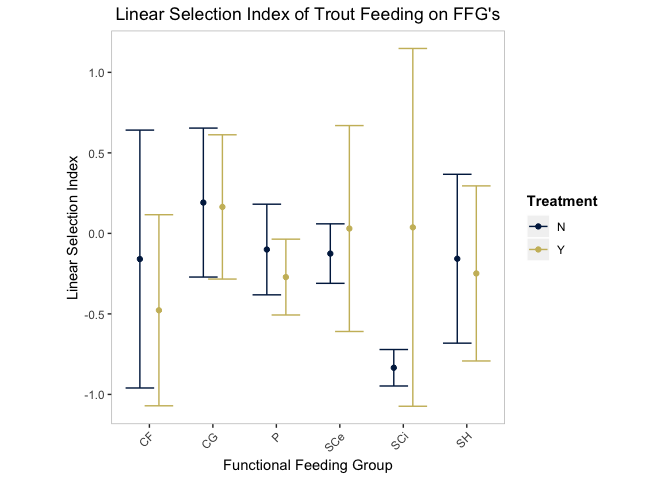
\includegraphics[width=4.16667in]{Figures/Diet-FFG-D-1.png}
  \caption{}
  \end{figure}
  
  \begin{figure}[htbp]
  \centering
  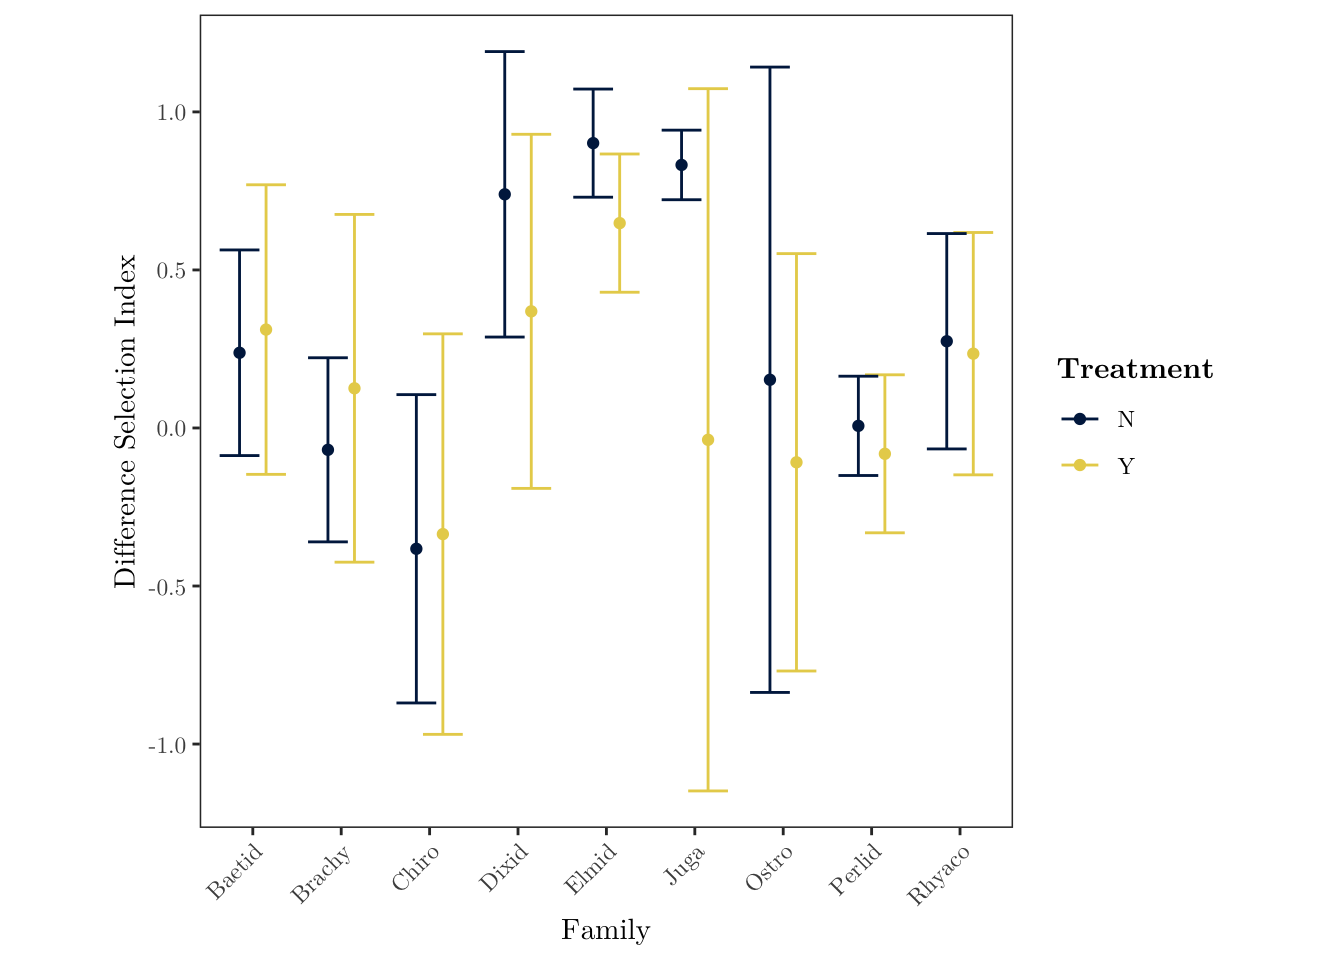
\includegraphics[width=4.16667in]{Figures/Diet-Fam-D-1.png}
  \caption{}
  \end{figure}
  
  \chapter*{Discussion}\label{discussion}
  \addcontentsline{toc}{chapter}{Discussion}
  
  Gaps are, by definition, patches in a larger, forested system.
  Therefore, significant localized responses to increases in light within
  a gap may not translate to significant system-wide responses at the
  stream or even the reach level. Our study design emphasizes the effects
  of gaps that comprise only a fraction of a stream reach, focusing on the
  integrated effect of small gaps embedded in a larger forested matrix.
  While light and Chla responded as expected to an opening of the riparian
  canopy, our reach-scale metrics for the invertebrate community do not
  show a response to increases in primary production. This does not match
  our original hypothesis that increases in high quality algae would lead
  to increased abundance of scraping invertebrate taxa. Instead, we find
  that the scale of the effect--increases in light are limited to within
  the gap--may outweigh the local magnitude. Even though algae is an
  energetically preferential food source, and primary production increased
  within treatment reaches, we see a limited invertebrate response at the
  reach level.
  
  The results for higher trophic levels seem to be in contradiction with
  previous studies on stream light (@ Heaston, Kaylor, Wooton), but these
  studies focused on
  
  Is a lack of system response to a local perturbation considered
  resilience?
  
  The overall response of the benthic invertebrate community to the canopy
  gaps was slight and indicates that no one species or functional group
  confers a competitive advantage from either increases in light or
  increased autochthonous production.
  
  When we replace taxonomy with functional groups, we still see no real
  changes in the relative abundance of functional feeding groups, which
  fits with our results from NMS.
  
  Trout diets also showed no response.
  
  The \emph{Juga} snail response fits our hypothesis, but hadn't been
  anticipated prior to field observations.
  
  Gap versus reach size. How large of a gap results in more than a
  local-within-gap response? When looking at a local response of grazers
  on tiles
  
  Power and Dietrich advocate for species exculsion studies to determine
  the top-down pressure of upper level consumers on lower members of the
  stream community (2002), but experimentally enhancing a particular basal
  resource can also reveal energy pathways and which community members are
  poised to take advantage of specific energy subsidies.
  
  In resiliency theory, the ability of a community to resist change is
  dependent on both the magnitude of disturbance and the degree of
  interspecific competition.
  
  \pagebreak
  
  \chapter*{References}\label{references}
  \addcontentsline{toc}{chapter}{References}
  
  \hypertarget{refs}{}
  \hypertarget{ref-Kaylor2017FS}{}
  Kaylor, M. J., Warren, D. R., \& Kiffney, P. M. (2017). Long-term
  effects of riparian forest harvest on light in pacific northwest (USA)
  streams. \emph{Freshwater Science}, \emph{36}(1), 1--13.
  
  \hypertarget{ref-Kreutzweiser2012}{}
  Kreutzweiser, D. P., Sibley, P. K., Richardson, J. S., \& Gordon, A. M.
  (2012). Introduction and a theoretical basis for using disturbance by
  forest management activities to sustain aquatic ecosystems.
  \emph{Freshwater Science}, \emph{31}(1), 224--231.
  
  \hypertarget{ref-Lau2009}{}
  Lau, D. C. P., Leung, K. M. Y., \& Dudgeon, D. (2009). What does stable
  isotope analysis reveal about trophic relationships and the relative
  importance of allochthonous and autochthonous resources in tropical
  streams? A synthetic study from hong kong. \emph{Freshwater Biology},
  \emph{54}(1), 127--141.
  
  \hypertarget{ref-Macarelli2011}{}
  Macarelli, A., \& others. (2011). Quantity and quality: Unifying food
  web and ecosystem perspectives on the role of resource subsidies in
  freshwater. \emph{Ecology}, \emph{92}, 1215--1225.
  
  \hypertarget{ref-PC-ORD}{}
  McCune, B., \& Mefford, M. J. (2016). \emph{PC-ord. multivariate
  analysis of ecological data. version 7.} Gleneden Beach, Oregon, U.S.A.:
  MjM Software Design.
  
  \hypertarget{ref-McCune2002}{}
  McCune, B., Grace, J. B., \& Urban, D. L. (2002). \emph{Analysis of
  ecological communities} (Vol. 28). MjM software design Gleneden Beach,
  OR.
  
  \hypertarget{ref-McCutchan2002}{}
  McCutchan, J. H. J., \& Lewis, W. M. J. (2002). Relative importance of
  carbon sources for macroinvertebrates in a rocky mountain stream.
  \emph{Limnology and Oceanography}, \emph{47}(3), 742--752.
  
  \hypertarget{ref-vegan}{}
  Oksanen, J., Blanchet, F. G., Friendly, M., Kindt, R., Legendre, P.,
  McGlinn, D., \ldots{} Wagner, H. (2018). \emph{Vegan: Community ecology
  package}. Retrieved from \url{https://CRAN.R-project.org/package=vegan}
  
  \hypertarget{ref-R-base}{}
  R Core Team. (2018). \emph{R: A language and environment for statistical
  computing}. Retrieved from \url{https://www.R-project.org/}
  
  \hypertarget{ref-Vannote1980}{}
  Vannote, R. L., Minshall, G. W., Cummins, K. W., Sedell, J. R., \&
  Cushing, C. E. (1980). The river continuum concept. \emph{Canadian
  Journal of Fisheries and Aquatic Sciences}, \emph{37}(1), 130--137.
  
  \hypertarget{ref-Wilzbach1986}{}
  Wilzbach, M. A., Cummins, K. W., \& Hall, J. D. (1986). Influence of
  habitat manipulations on interactions between cutthroat trout and
  invertebrate drift. \emph{Ecology}, \emph{67}(4), 898--911.


\end{document}

